\documentclass{beamer}
\usetheme{Madrid}

\beamertemplatenavigationsymbolsempty

\definecolor{fore}{RGB}{249,242,215}
\definecolor{back}{RGB}{51,51,51}
\definecolor{title}{RGB}{60,230,60}
\definecolor{tback}{RGB}{150,10,10}

\setbeamercolor{titlelike}{fg=title,bg=tback}
\setbeamercolor{normal text}{fg=fore,bg=back}

\usepackage{listings,times}
\usepackage{fontspec}
\definecolor{keywords}{RGB}{30,200,30}
\definecolor{comments}{RGB}{210,40,40}
\lstset{language=Haskell,
breaklines=true,
basicstyle=\ttfamily\small,
showstringspaces=false,
keywordstyle=\color{keywords},
commentstyle=\color{comments}\emph}

\title{Transformatory monad}
\subtitle{Czyli jak łatwo pisać modularne programy}
\author{Łukasz Czapliński}
\date{\today}

\begin{document}

\maketitle

\begin{frame}[fragile] % (fold)
  \frametitle{Szybkie przypomnienie}
    \begin{itemize}
      \item Monady to ,,design pattern'' programowania funkcyjnego.
      \item Pozwalają operować na jednym z elementów pudełka (funktora) bez
                    znajomości jego struktury (\texttt{>>=}).
      \item Pozwalają na modelowanie efektów w czystym języku funkcyjnym (np. stanu).
    \end{itemize}
\end{frame}

\begin{frame}{Prawa monadyczne}
  \begin{itemize}
    \item \texttt{return >=> f = f}
    \item \texttt{f >=> return = f}
    \item \texttt{a >=> (b >=> c) = (a >=> b) >=> c}
    \pause
    \item Monoid! Operacja łączna z elementem neutralnym.
    \item (\texttt{g :: Functor f => a -> f b} nazywamy endofunktorem)
  \end{itemize}
\end{frame}


\begin{frame} % (fold)
  \frametitle{Cel na dzisiaj}
  Napisać interpreter prostego języka o następujących cechach:
  \begin{itemize}
    \item posiada zmienne,
    \item występują funkcje,
    \item obsługuje operacje logiczne.
  \end{itemize}
  Dlaczego interpreter? Bo da się przenieść na dowolny inny program.
\end{frame}

\begin{frame}[fragile] % (fold)
  \frametitle{Jak interpretować?}
\begin{lstlisting}
data Term = And Term Term | Or Term Term 
  | Var Variable | Not Term 
  | Let Variable Term Term | Const Value
  | Appl Function Term deriving (Read, Show, Ord, Eq)

interp :: InterpMonad m => Term -> m Value
\end{lstlisting}
\end{frame}

\begin{frame}[fragile] % (fold)
  \frametitle{Czym jest InterpMonad?}
\begin{lstlisting}
class (MonadState m, MonadEnv m) => InterpMonad m where
  start :: (Show a, InterpMonad m) => m a -> String
\end{lstlisting}
\end{frame}

\begin{frame}[fragile] % (fold)
  \frametitle{Monada stanowa}
\begin{lstlisting}
class Monad m => MonadState m where
  modState :: (State -> State) -> m State
  putVar :: Variable -> Term -> m ()
  getVar :: Variable -> m (Maybe Term)
\end{lstlisting}
\end{frame}

\begin{frame}[fragile] % (fold)
  \frametitle{Monada środowiskowa}
\begin{lstlisting}
class Monad m => MonadEnv m where
  parseEnv :: String -> m (Maybe Env)
  inEnv :: Env -> m a -> m a
  lookupEnv :: Function -> m (Maybe Func)
\end{lstlisting}
\end{frame}

\begin{frame}[fragile] % (fold)
  \frametitle{Implementacja - podejście 1: wprost.}
\begin{lstlisting}
newtype StateC a = StateC { runStateC:: State -> (State, a) }

instance Monad StateC where
  return x = StateC $ \s -> (s,x) 
  m >>= f = StateC $ (\s -> let (s',a) = runStateC m $ s in runStateC (f a) $ s')

instance MonadState StateC where
  modState f = StateC $ \s -> (f s, s)
  putVar v t = modState (putState v t) >> return ()
  getVar v = StateC $ \s -> (s, lookup v s)
\end{lstlisting}
Podobnie dla MonadEnv.
\end{frame}

\begin{frame}[fragile] % (fold)
  \frametitle{Dla ciekawskich: MonadEnv}
  \begin{lstlisting}
  newtype EnvC a = EnvC { runEnvC :: Env -> a }

  instance Monad EnvC where
    return x = EnvC $ \_ -> x
    m >>= f = EnvC $ \r -> runEnvC (f (runEnvC m $ r)) $ r

  instance MonadEnv EnvC where
    parseEnv = return.strToEnv   
    inEnv e f = return $ runEnvC f e
    lookupEnv f = EnvC $ \r -> lookup f r 
  \end{lstlisting}
\end{frame}

\begin{frame}[fragile] % (fold)
  \frametitle{Dygresja: podział pracy na monady}
  \begin{itemize}
    \item Modularyzacja
    \item Trudniej o błedy
    \item Prostsze struktury danych
    \item Mozliwość kontroli zachowania
  \end{itemize}
\end{frame}

\begin{frame}[fragile] % (fold)
  \frametitle{Składanie w całość}
\begin{lstlisting} % (fold)

newtype OurMonad a = OurMonad { runO:: EnvC (StateC a) }
-- EnvC (Env -> StateC (State -> (State, a)))
instance Monad OurMonad where
  return x = OurMonad $ return $ return x
  m >>= f = OurMonad $ EnvC ( \r -> runEnvC (runO m) r >>= (\a -> runEnvC (runO (f a)) r))

\end{lstlisting}
\end{frame}

\begin{frame}[fragile] % (fold)
  \frametitle{A może by tak dodać obsługę błędów?}
\begin{lstlisting}

class Monad m => MonadError m where
  err :: Error -> m a
newtype OurMonad a = OurMonad { runO:: EnvC (StateC (ErrorC a)) }
-- EnvC (Env -> StateC (State -> (State, ErrorC (Either Err a)))

\end{lstlisting}
Nowy bind - ile trzeba zmienić?
Za dużo.
\end{frame}

\begin{frame}[fragile] % (fold)
  \frametitle{Co można zmienić?}
  Co chcielibyśmy otrzymać?\\
  $\rightarrow$ Możliwość składania monad. Możemy to uzyskać np: używając w definicji bind bind monady bazowej. \\
  Co jeśli w wyniku nie będzie monady?\\
  $\rightarrow$ Stwórzmy sztuczną: Monad Id
  \begin{lstlisting} % (fold)

newtype Id a = Id { runId :: a }
instance Monad Id where
  return = Id
  m >>= f = f (runId m)

  \end{lstlisting}
\end{frame}

\begin{frame}[fragile] % (fold)
  \frametitle{Podsumowanie}
  Teraz możemy być pewni, że nasza monada jako typ wynikowy będzie miała pewną monadę. Wobec tego możemy w definicji bind użyc bind monady wynikowej.
  Otrzymujemy typ: 
  \begin{lstlisting} % (fold)

  Monad m => Monad (t m)

  \end{lstlisting}
  gdzie t jest tworzonym przez nas typem. Stąd nazwa transformatory monad.
\end{frame}

\begin{frame}[fragile] % (fold)
  \frametitle{Transformatory monad - formalniej}
  \begin{itemize}
    \item mają typ (*->*) -> *->*
    \item jeśli argumentem jest monada, to wynikiem też.
  \end{itemize}
\end{frame}

\begin{frame}[fragile] % (fold)
  \frametitle{Przykład 1: StateT}
  \begin{lstlisting} % (fold)

newtype StateT m a = StateT { runStateT :: State -> m (State,a) }
instance Monad m => Monad (StateT m) where
  return x = StateT $ \s -> return (s,x)
  m >>= f = StateT $ \s -> do
    (s',a) <- runStateT m s
    runStateT (f a) s'

instance Monad m => MonadState (StateT m) where
  modState f = StateT $ \s -> return (f s, s)
  putVar v t = modState (putState v t) >> return ()
  getVar v = StateT $ \s -> return (s, lookup v s)

  \end{lstlisting}
\end{frame}

\begin{frame}[fragile] % (fold)
  \frametitle{Przykład 2: Env}
  \begin{lstlisting} % (fold)

newtype EnvT m a = EnvT { runEnvT :: Env -> m a }
instance Monad m => Monad (EnvT m) where
  return x = EnvT $ \_ -> return x
  m >>= f = EnvT $ \e -> do
    a <- runEnvT m e
    runEnvT (f a) e

instance Monad m => MonadEnv (EnvT m) where
  parseEnv =  return.strToEnv
  inEnv e f = EnvT $ \_ -> runEnvT f e
  lookupEnv f = EnvT $ \e -> return $ lookup f e

  \end{lstlisting}
\end{frame}

\begin{frame}[fragile] % (fold)
  \frametitle{Niespodziewany problem}
  \framesubtitle{Jak teraz podnieść obliczenia w monadzie bazowej?}
    Przedtem wystarczyło zrobić return.\\
    Teraz: \ttfamily{return :: a -> (t m ) a}, a potrzeba \ttfamily{lift :: m a -> (t m) a}
  \begin{lstlisting} % (fold)

class MonadT t where
  lift :: Monad m => m a -> t m a

instance MonadT StateT where
  lift m = StateT $ \s -> do
    a <- m
    return (s,a)

instance MonadT EnvT where
  lift m = EnvT $ \_ -> m

  \end{lstlisting}
  To po prostu return na resorach.
\end{frame}

\begin{frame}[fragile] % (fold)
  \frametitle{Podejście 2: z transformatorami}
  \begin{lstlisting} % (fold)

  newtype OurMonad a = OurMonad { runO :: EnvT (StateT (Id)) a } 
  liftFromEnv :: EnvT (StateT (Id)) a -> OurMonad a
  liftFromEnv = OurMonad
  liftFromState :: StateT (Id) a -> OurMonad a
  liftFromState = liftFromEnv.lift

  instance Monad OurMonad where
    return = OurMonad . return 
    m >>= f = OurMonad $ do
      a <- runO m
      runO $ f a

  \end{lstlisting}
\end{frame}

\begin{frame}[fragile] % (fold)
  \frametitle{Dodajmy error}
  \begin{lstlisting} % (fold)

newtype OurMonad a = OurMonad { runO :: ErrorT (EnvT (StateT (Id))) a } 
liftFromErr :: ErrorT (EnvT (StateT (Id))) a -> OurMonad a
liftFromErr = OurMonad 
liftFromEnv :: EnvT (StateT (Id)) a -> OurMonad a
liftFromEnv = liftFromErr.lift
liftFromState :: StateT (Id) a -> OurMonad a
liftFromState = liftFromEnv.lift

instance Monad OurMonad where
  return = OurMonad . return 
  m >>= f = OurMonad $ do
    a <- runO m
    runO $ f a

  \end{lstlisting}
  Właściwie bez zmian!
\end{frame}

\begin{frame}[fragile] % (fold)
  \frametitle{Dokończmy implementację}
  \begin{lstlisting} % (fold)

instance MonadError OurMonad where
  err str = liftFromErr $ err str

instance MonadState OurMonad where
  modState f = liftFromState $ modState f
  putVar v t = liftFromState $ putVar v t
  getVar v = liftFromState $ getVar v

instance MonadEnv OurMonad where
  inEnv e f = liftFromErr $ ErrorT $ inEnv e $ runErrorT $ runO f 
  parseEnv s = liftFromEnv $ parseEnv s
  lookupEnv f = liftFromEnv $ lookupEnv f

  \end{lstlisting}
\end{frame}

\begin{frame}[fragile] % (fold)
  \frametitle{Pozostaje formalność}
  \begin{lstlisting} % (fold)

instance InterpMonad OurMonad where
  start o = case runId $ runStateT (runEnvT (runErrorT $ runO o) basicEnv) basicState of
  (s, Left err) -> "Error: " ++ err ++ " in state:[ " ++ show s ++ " ]"
    (_,Right a) -> show a

  \end{lstlisting}
  Teraz mamy gotowy interpreter.
\end{frame}

\begin{frame} % (fold)
  \frametitle{Pułapki}
  \begin{itemize}
    \item kolejność składania $\rightarrow$ StateT (ErrorT Id) a czy ErrorT (StateT Id) a?
    \item monada listowa $\rightarrow$ odpowiedni transformator
    \item lift $\rightarrow$ co jeśli chcemy podnieść funkcję?
  \end{itemize}
\end{frame}

\begin{frame}[fragile] % (fold)
  \frametitle{Kolejność składania monad}
  \begin{lstlisting} % (fold)
  
  StateT (ErrorT Id) a
  State -> Either Err (State,a)

  ErrorT (StateT Id) a
  State -> (State, Either Err a)

  \end{lstlisting}
  Otrzymujemy inne właściwości monady wynikowej. 
\end{frame}

\begin{frame}[fragile] % (fold)
  \frametitle{Monada listowa}
  \begin{lstlisting} % (fold)

  class Monad m => MonadList m where
    merge :: m a -> m a -> m a

  instance Monad m => MonadList (t m) where
    merge :: (t m) a -> (t m) a -> (t m) a

  \end{lstlisting}
\end{frame}

\begin{frame}[fragile] % (fold)
  \frametitle{LiftT z Control.Monad.Trans.List}
\begin{lstlisting} % (fold)

newtype ListT = ListT { runListT :: m [a] }

test1 :: ListT IO Int
test1 = do
  r <- liftIO (newIORef 0)
  (next r `mplus` next r >> next r `mplus` next r) >> next r `mplus` next r
 
test2 :: ListT IO Int
test2 = do
  r <- liftIO (newIORef 0)
  next r `mplus` next r >> (next r `mplus` next r >> next r `mplus` next r)
 
next :: IORef Int -> ListT IO Int
next r = liftIO $ do  x <- readIORef r
                      writeIORef r (x+1)
                      return x
\end{lstlisting}
\end{frame}

\begin{frame}[fragile] % (fold)
  \frametitle{Wyniki}
  \begin{lstlisting} % (fold)

main = do
  arg <- getArgs
  case head arg of 
    "1" -> runListT test1
    _   -> runListT test2

$ runghc example.hs 1
[6,7,8,9,10,11,12,13]
$ runghc example.hs 2
[4,5,6,7,10,11,12,13]

  \end{lstlisting}
\end{frame}

\begin{frame}[fragile] % (fold)
  \frametitle{ListT done right?}
  \begin{lstlisting} % (fold)

  -- The monadic list type
  data MList' m a = MNil | a `MCons` MList m a
  type MList m a  = m (MList' m a)
   
  -- This can be directly used as a monad transformer
  newtype ListT m a = ListT { runListT :: MList m a }
   
  -- A "lazy" run function, which only calculates the first solution.
  runListT' :: Functor m => ListT m a -> m (Maybe (a, ListT m a))
  runListT' (ListT m) = fmap g m where
    g MNil = Nothing
    g (x `MCons` xs) = Just (x, ListT xs)

  \end{lstlisting}
\end{frame}

\begin{frame}[fragile] % (fold)
  \frametitle{...i jego problem}
  \begin{lstlisting} % (fold)

  test = runListT $ do
    x <- liftList [1..3]
    liftIO $ print x
    y <- liftList [6..8]
    liftIO $ print (x,y)

  \end{lstlisting}
\end{frame}

\begin{frame}[fragile] % (fold)
  \begin{tabular}{l|l}
  
  \begin{lstlisting} % (fold)

  Using Control.Monad.List:
  Main> test
  1
  (1,6)
  (1,7)
  (1,8)
  2
  (2,6)
  (2,7)
  (2,8)
  3
  (3,6)
  (3,7)
  (3,8)

  \end{lstlisting}&
  \begin{lstlisting}

  Using "ListT done right":
  Main> test
  1
  (1,6)

  \end{lstlisting}
  \end{tabular}
\end{frame}

\begin{frame}[fragile]
  \frametitle{Rozwiązanie}
  Wobec tego najprościej nie używać transformatora, użyć [] zamiast Id jako monady bazowej.\\
  \begin{lstlisting} % (fold)

  newtype OurListMonad a = OLM { runOLM::ErrorT (StateT []) a}
  -- State -> [(State, Either Err a)]

  \end{lstlisting}
  Wówczas merge to dodanie odpowiednich list.
  Niestety wówczas rezygnujemy ze skutków ubocznych: nie możemy użyć IO jako monady bazowej. Co oddaje istotę powyższego problemu.
\end{frame}

\begin{frame}[fragile] % (fold)
  \frametitle{Trochę formalności: lift}
  Jak powinien działać?\\
  Prawa\\
  \begin{itemize}
    \item \ttfamily{lift . return = return}
    \item \ttfamily{lift (m `bind` k) = (lift m) `bind` (lift . k)} 
  \end{itemize}
\end{frame}

\begin{frame}[fragile] % (fold)
  \frametitle{Lift}
  \begin{center}
    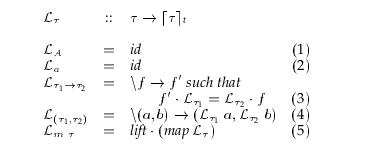
\includegraphics[scale=0.6]{images/Constraint.png} \\
    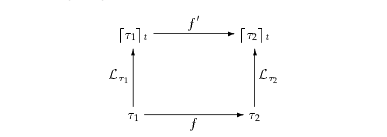
\includegraphics[scale=0.6]{images/Graph.png}
  \end{center}
  {\tiny From Monad Transformers and Modular Interpreters (Sheng Liang
  Paul Hudak
Mark Jones).}
\end{frame}

\begin{frame} % (fold)
  \begin{center}
    {\huge Pytania i uwagi?}
    
    \begin{itemize}
      \item Jak połączyć IO z monadami? $\rightarrow$ piszemy grę
      \item Jak połączyć IO z różnymi wynikami? $\rightarrow$ piszemy Prologa
    \end{itemize}
  \end{center}
\end{frame}

\begin{frame}[fragile] % (fold)
  \frametitle{Zadanie}
  \begin{lstlisting} % (fold)

data Term = And Term Term | Or Term Term 
  | Var Variable | Not Term 
  | Let Variable Term Term | Const Value
  | Twofold Variable Term  deriving (Read, Show, Ord, Eq)

  interp Twofold v t -> do
    mv <- getVar v
    if mv /= Nothing
      then err $ "Variable " ++ v ++ " already taken at this point."
      else return ()
    let v1 = branch v True t
    let v2 = branch v False t
    merge v1 v2

  \end{lstlisting}
\end{frame}


\begin{frame}[fragile] % (fold)
  \frametitle{Zadanie - c.d.}
  \begin{lstlisting} % (fold)

class (MonadState m, MonadWriter m, MonadList m, MonadError m) => InterpMonad m where
  start :: (Show a, InterpMonad m) => m a -> String

class Monad m => MonadWriter m where
  tell :: String -> m ()

  \end{lstlisting}
\end{frame}

\begin{frame}[fragile] % (fold)
  \frametitle{Przykład}
  \begin{verbatim}

    --term4:
    Twofold "x" 
      (Twofold "y" 
        (Or 
          (Or 
            (Let "x" (Const False) (Var"x")) 
            (Var "y")) 
          (Var"z")))

\end{verbatim}
\end{frame}

\begin{frame}[fragile] % (fold)
  \frametitle{Przykład}
  \tiny{
  \begin{center}
  \begin{tabular}{ p{0.45\textwidth} | p{0.45\textwidth}}
    \begin{lstlisting}
Testing x as True..
Testing y as True..
Warning: overwriting var x .
Done with y.
Done with x.
---- Answer: True
Testing x as True..
Testing y as False..
Warning: overwriting var x .
Something went wrong..
 No such variable as z at this point.
{State: [("x",Const True),("y",Const False)]}
     \end{lstlisting}
     &
     \begin{lstlisting}
Testing x as False..
Testing y as True..
Warning: overwriting var x .
Done with y.
Done with x.
---- Answer: True
Testing x as False..
Testing y as False..
Warning: overwriting var x .
Something went wrong..
 No such variable as z at this point.
{State: [("x",Const False),("y",Const False)]}
    \end{lstlisting}
  \end{tabular}
\end{center}
}
\end{frame}

\begin{frame} % (fold)
  \begin{center}
    \huge{Dziekuję za uwagę}
  \end{center}
\end{frame}

\end{document}

